\documentclass{article}

\usepackage{amsmath}
\usepackage[utf8]{inputenc} 
\usepackage[serbian]{babel} 
\usepackage{hyperref} 
\usepackage{graphicx} 
\usepackage{listings} 
\usepackage{tikz}
\usepackage{color, colortbl}
\usepackage[backend=biber]{biblatex}
\usepackage[nottoc]{tocbibind}
\graphicspath{ {./images/} }
\usepackage{caption}
\usepackage{subcaption}
\usepackage[T1]{fontenc}
\definecolor{Gray}{gray}{0.9}
\usepackage{hyperref}
\hypersetup{
colorlinks,
linkcolor=blue,
urlcolor=blue
}
\setlength{\textheight}{600pt}
\setlength{\textwidth}{140mm}
\setlength{\topmargin}{5pt}
\setlength{\evensidemargin}{53pt}
\setlength{\oddsidemargin}{10mm}

\addbibresource{references.bib}

\title{%
  Rešavanje slagalice primenom genetskog algoritma \vspace{0.4cm} \\ 
  \large Projekat u okviru kursa Računarska inteligencija \\
  Matematički fakultet\\ Univerzitet u Beogradu \vspace*{0.5cm}}
  
\author{Lazar Čeliković \\
\href{mailto:celikoviclazar@hotmail.com}{celikoviclazar@hotmail.com} \\
Miloš Milakovič \\
\href{mailto:mi17152@alas.matf.bg.ac.rs}{mi17152@alas.matf.bg.ac.rs} \\
}

\date{\vspace*{1cm}Avgust 2021}


\begin{document}
  \maketitle
  \newpage
  \renewcommand*\contentsname{Sadržaj}
  \tableofcontents{}
  \newpage
\section{Opis problema}
Problem koji se u ovom radu rešava jeste problem slaganja slagalice. Na ulazu se dobija niz izmešanih delova i cilj je složiti sve delove na svoje mesto. U ovom radu je dat postupak implementacije automatizacije ovog procesa pomoću genetskog algoritma.

\section{Implementacija}

\subsection{Obrada ulaznih podataka}

Na ulazu u algoritam dobijamo fotografiju od koje želimo da napravimo slagalicu. Takođe, među parametrima zadajemo i dimenzije jednog dela. Uz pomoć tog parametra sečemo sliku i na taj način formiramo niz delova slagalice. Taj niz nam postaje ulaz u genetski algoritam.
Svaki deo je predstavljen kao matrica piksela. Dakle, za svaki piksel pamtimo njegovu RGB vrednost i te informacije koristimo za kalkulaciju fitnesa što će biti objašnjeno kasnije u radu.

\subsection{Genetski algoritam}
\subsubsection{Uopšteno o algoritmu}
Osnovna ideja genetskog algoritma meže se opisati u nekoliko koraka:\newline
\newline
1. Definisanje svih potrebnih parametara problema i genetskog algoritma\newline
2. Formiranje inicijalne populacije\newline
3. Dekodiranje hromozoma — ovaj korak se javlja samo kod binarnih GA\newline
4. Određivanje cena hromozomima (fitnes funkcijom)\newline
5. Selekcija hromozoma koji će postati ulaz za fazu ukrštanja\newline
6. Ukrštanje — iz populacije se izdvajaju dva hromozoma (roditelji) i njihov genetski materijal se ukršta. Kao proizvod tog ukrštanja nastaje jedan ili više potomaka koji bi trebalo da imaju bolji genetski materijal (u terminima fitnes funkcije) od roditelja\newline
7. Mutacije, pri kojima se menja genetski sadržaj hromozoma\newline
8. Ispitivanje konvergencije, da bi se utvrdilo da li ima osnova da se tok algoritma prekine. Ukoliko nije ispunjen uslov konvergencije, vratiti se na korak 3 odnosno 4.\newline


\subsubsection{Implementacija jedinke}
Svaka jedinka, odnosno hromozom predstavljen je kao objekat koji sadrži niz elemenata slagalice. Dakle, hromozom predstavlja jedno potencijalno rešenje slagalice. Inicijalna populacija onda predstavlja niz potencijalnih rešenja. Ona se kreira tako što se napravi niz delova od ulazne fotografije i onda se od tog niza pravi potreban broj jedinki nasumičnim mešanjem tih delova.\newpage
Takođe, svaka jedinka ima polje koje predstavlja vrednost fitnes funkcije. Ta vrednost označava koliko je ta konkretna jedinka dobra, odnosno koliko je bliska polaznoj fotografiji u našem slučaju. Ideja za računanje ove vrednosti korišćena u našoj implementaciji jeste da se svaki deo poredi sa svojim susedima, odnosno da im se porede ivice. Intuicija iza ovoga jeste da ako delovi treba da stoje jedan pored drugoga onda bi RGB vrednosti trebalo da im budu slične. Dakle, fitnes funkcija se računa oduzimanjem RGB vrednosti za dve ivice i sabiranjem.\newline

$$f(x) = \sum(((w1- w2)/255)^2)$$

U prethodnoj formuli w1 i w2 predstavljaju ivice nekog dela slagalice. Deljenje sa 255 koristimo da bismo doveli vrednosti RBG za piksele na interval [0, 1]. Dakle, što je vrednost fitnes funkcije manja veća je verovatnoća da je ta jedinka naše rešenje.

\subsubsection{Selekcija, ukrštanje, elitizam}
Prilikom implementacije podržana je i turnirska i ruletska selekcija. Parametre koje koristimo prilikom vršenja selekcije prosleđujemo algoritmu na početku.\newline\newline
Ukrštanje je posebno zanimljivo u ovom slučaju. Ideja je da se uzmu dve jedinke i da se od njih ukrštanjem pravi jedan potomak. Izazov ovde jeste u tome što moramo da budeo vrlo pažljivi koje delove ubacujemo u jezgro jer može vrlo lako da se desi da ubacimo isti deo iz oba roditelja i onda narušavamo inicijalnu strukturu jedinke. Proces ukrštanja jedinki sastoji se iz tri faze. Sada ćemo ih ukratko opisati.\newline\newline
Prva faza se sastoji od sledećeg. Naime, krećemo od proizvoljnog dela jednog roditelja i tražimo sve susede tog dela koji su isti kod oba roditelja. Intuicija iza ovog postupka jeste u tome da ako se delovi kod oba roditelja nalaze jedni pored drugih veća je verovatnoća da je to korektan raspored. Rezultat ove faze biće jezgro koje predstavlja matricu delova. Vrlo je verovatno da će neka polja u jezgru ostati nepopounjena. To se rešava u narednim fazama.\newline\newline
Druga faza podrazumeva traženje takozvanog best buddy dela. Naime, kada smo dobili jezgro koje čine delovi koji su isto raspoređeni kod oba roditelja prelazimo na traženje onih delova koji se najbolje uklapaju sa već složenim delovima. Kada pronađemo deo za koji smatramo da je najbolji za tu poziciju ubacujemo ga na istu. I ovde kao i u prethodnoj fazi moramo da vodimo računa o granicama jezgra koje konstantno raste. Znamo da je slagalica dimenzija nxm i samim tim moramo da pazimo da rezultat ukrštanja takođe bude tih dimenzija. Na primer, ako želimo da ubacimo deo desno od najdešnjeg dela u jezgru, moramo da proverimo da li ta pozicija upada u granice jezgra. Ako ne, pokušavamo da transliramo sve deloje u levo za jednu poziciju ako je to moguće. Ukoliko je to moguće, ubacujemo izabrani deo na najdešnju poziciju i nastavljamo dalje. Ukoliko transliranje nije bilo moguće jednostavno vraćamo taj deo među neraspoređene i nastavljamo sa algoritmom.\newline\newline
Treća faza podrazumeva uzimanje preostalih delova i nasumično raspoređivanje na preostala slobodna mesta u jezgru.\newline\newline
Nakon ovoga dobijamo novu jedinku koja takođe ima niz delova slagalice. Sam postupak nam garantuje da će dimenzije novonastale jedinke odgovarati domenzijama roditelja kao i to da će se svaki deo naći u novonastaloj jedinci tačno jednom.\newline
\newline
Elitizam je realizovan pre procesa selekicje. Automatski je uzeto n jedinki i one su ubačene u narednu generaciju. Nakon toga se proces selekcije primenjuje na preostale jedinke. Takođe, među parametrima algoritma se može zadati broj jedinki za elitizam kao i opcija da ne želimo da imamo elitizam uopšte.

\subsubsection{Parametri genetskog algoritma}
Parametri za ovaj algoritam se prosleđuju prilikom pokretanja komande iz terminala. U odeljku koji se bude bavio analizom rezultata će biti prikazano kako se algoritam ponaša za različite vrednosti parametara. Neki od parametara koji se mogu zadavati su broj generacija, broj jedinki za elitizam, veličina populacije, tip selekcije i veličina dela slagalice.

\subsection{Izlaz programa}
Kada se algoritam završi kao rezultat dobijamo fotografiju koja se dobija spajanjem svih delova slagalice. Pored potografije, program nam ispisuje još neke korisne statistike kao što je vreme koje je bilo potrebno da se dođe do rešenja, da li se algoritam zaustavio ranije jer je iskonvergirao... Ove statistike će biti korišćenje u odeljku koji se bavi prikazivanjem i analizom rezultata.

\addcontentsline{toc}{section}{Rezultati}
\section{Rezultati}

Sledi par primera rešavanja slagalice i prikaz izgleda slagalice u određenim generacijama.

\begin{figure}[h]
     \centering
	 \captionsetup{justification=centering}
     
     \begin{subfigure}[t]{0.3\textwidth}
         \centering
         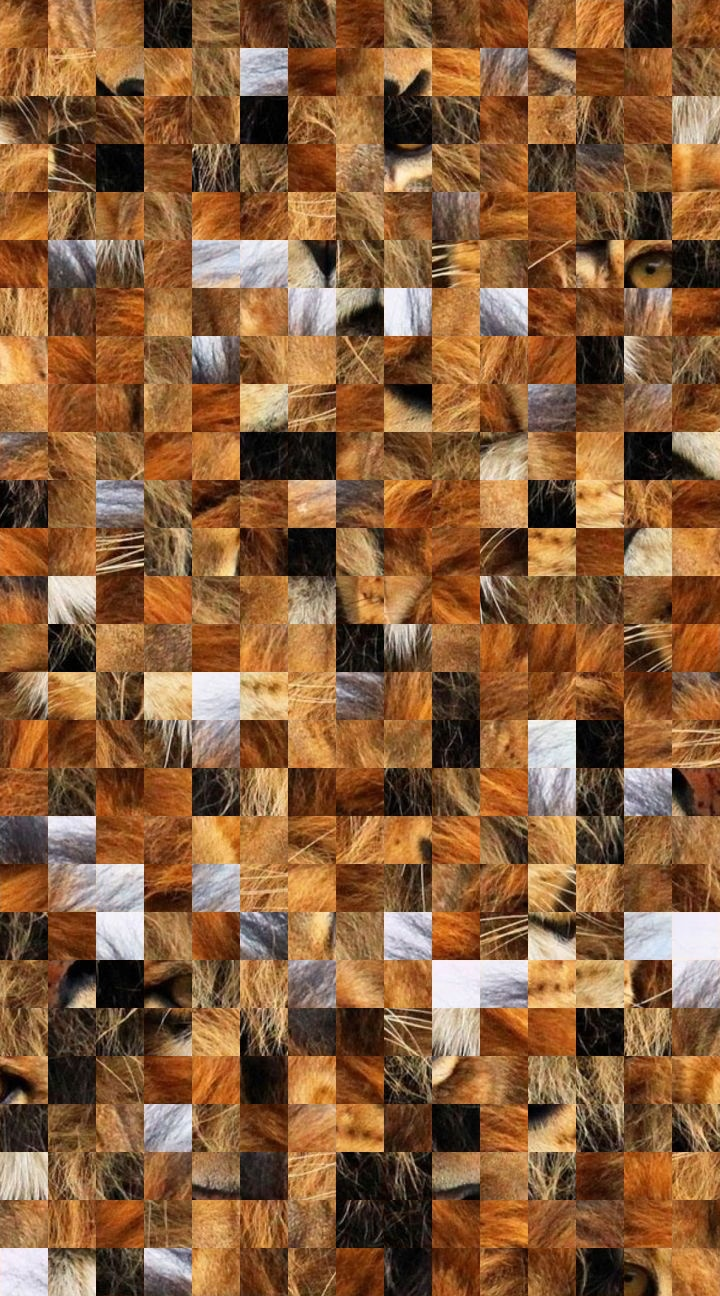
\includegraphics[width=\textwidth]{lav_48_pocetak}
         \caption{{Početni izgled slagalice}}
         \label{fig:lav_48_pocetak}
     \end{subfigure}
     \hfill
     \begin{subfigure}[t]{0.3\textwidth}
         \centering
         \includegraphics[width=\textwidth]{lav_48_generacija_1}
         \caption{{Najbolja jednika u generaciji 1}}
         \label{fig:lav_48_generacija_1}
     \end{subfigure}
     \hfill
     \begin{subfigure}[t]{0.3\textwidth}
         \centering
         \includegraphics[width=\textwidth]{lav_48_generacija_3}
         \caption{{Krajnje rešenje se dostiže u trećoj generaciji}}
         \label{fig:lav_48_generacija_3}
     \end{subfigure}
     
     \caption{\textit{Primer rešavanja slagalice lava. Veličina dela je 48x48 piksela a broj delova slagalice je 405. Potrebno vreme da reši je 66.153 sekunde.}}
\end{figure}
\clearpage
\begin{figure}[h]
     \centering
	 \captionsetup{justification=centering}
     
     \begin{subfigure}[t]{0.3\textwidth}
         \centering
         \includegraphics[width=\textwidth]{lav_30_pocetak}
         \caption{{Početni izgled slagalice}}
         \label{fig:lav_30_pocetak}
     \end{subfigure}
     \hfill
     \begin{subfigure}[t]{0.3\textwidth}
         \centering
         \includegraphics[width=\textwidth]{lav_30_generacija_1}
         \caption{{Najbolja jednika u generaciji 1}}
         \label{fig:lav_30_generacija_1}
     \end{subfigure}
     \hfill
     \begin{subfigure}[t]{0.3\textwidth}
         \centering
         \includegraphics[width=\textwidth]{lav_30_generacija_2}
         \caption{{Najbolja jednika u generaciji 2}}
         \label{fig:lav_30_generacija_2}
     \end{subfigure}
     \begin{subfigure}[t]{0.3\textwidth}
         \centering
         \includegraphics[width=\textwidth]{lav_30_generacija_3}
         \caption{{Najbolja jednika u generaciji 3}}
         \label{fig:lav_30_generacija_3}
     \end{subfigure}
     \begin{subfigure}[t]{0.3\textwidth}
         \centering
         \includegraphics[width=\textwidth]{lav_30_kraj}
         \caption{{Krajnje rešenje}}
         \label{fig:lav_30_kraj}
     \end{subfigure}
     
     \caption{\textit{Primer rešavanja slagalice lava. Veličina dela je 30x30 piksela a broj delova slagalice je 1032. Potrebno vreme da reši je 230.02 sekunde.}}
\end{figure}
\clearpage

Naredni primer je primer slagalice u kojoj prilikom rešavanja dolazi do problema jer su svuda boje slične i ne može da se napravi jasna razlika između delova.
\begin{figure}[h]
     \centering
	 \captionsetup{justification=centering}
     
     \begin{subfigure}[t]{0.3\textwidth}
         \centering
         \includegraphics[width=\textwidth]{night_sky_48_pocetak}
         \caption{{Početni izgled slagalice}}
         \label{fig:night_sky_48_pocetak}
     \end{subfigure}
     \hfill
     \begin{subfigure}[t]{0.3\textwidth}
         \centering
         \includegraphics[width=\textwidth]{night_sky_48_generacija_1}
         \caption{{Najbolja jednika u generaciji 1}}
         \label{fig:night_sky_48_generacija_1}
     \end{subfigure}
     \hfill
     \begin{subfigure}[t]{0.3\textwidth}
         \centering
         \includegraphics[width=\textwidth]{night_sky_48_generacija_2}
         \caption{{Najbolja jednika u generaciji 2}}
         \label{fig:night_sky_48_generacija_2}
     \end{subfigure}
     \begin{subfigure}[t]{0.3\textwidth}
         \centering
         \includegraphics[width=\textwidth]{night_sky_48_generacija_3}
         \caption{{Najbolja jednika u generaciji 3}}
         \label{fig:night_sky_48_generacija_3}
     \end{subfigure}
     \begin{subfigure}[t]{0.3\textwidth}
         \centering
         \includegraphics[width=\textwidth]{night_sky_48_kraj}
         \caption{{Krajnje rešenje}}
         \label{fig:night_sky_48_kraj}
     \end{subfigure}
     
     \caption{\textit{Primer rešavanja slagalice noćnog neba. Veličina dela je 48x48 piksela a broj delova slagalice je 216. Potrebno vreme da reši je 70.481 sekunde.}}
\end{figure}

U zavisnosti od broja delova slagalice algoritmu će biti potrebno više ili manje vremena da reši slagalicu. Takođe povećavanjem broja generacija i jedinki u generaciji može da se dobije bolje rešenje ali će isto tako i vreme izvršavanja programa da raste.
Mi smo testirali ove primere sa 20 generacija i 600 jedinki u jednoj generaciji.

\section{Zaključak}
Na osnovu rezultata iz prethodnog odeljka možemo zaključiti da naša implementacija ovog algoritma daje zadovoljavajuće rezultate. Za veliki broj ulaznih fotografija se dobija perfektno složena slika, međutim postoje i slučajevi kada rešenje i nije tako dobro. Primer takvog slučaja jeste kada imamo deo slike koji je veoma monoton, odnosno jednobojan. Algoritam tu vidi da su RGB vrednosti slične i uklapa te elemente. Problem je što u većini slučajeva ispermutuje te elemente odnosno ne može da odredi tačne pozicije tih elemenata jer su svi prilično slični. Ovo jeste veoma lep prostor za modifikaciju i dalje unapređivanje ovog algoritma. 
\newpage

\begin{thebibliography}{8}

\bibitem{Drugi} 
\href{https://openaccess.thecvf.com/content_cvpr_2013/papers/Sholomon_A_Genetic_Algorithm-Based_2013_CVPR_paper.pdf}{A Genetic Algorithm-Based Solver for Very Large Jigsaw Puzzles}
\bibitem{Springer} 
\href{https://link.springer.com/chapter/10.1007/978-3-030-53956-6_32}{A Genetic Algorithm-Based Solver for Small-Scale Jigsaw Puzzles}
\bibitem{Treci} 
\href{https://web.stanford.edu/class/cs231a/prev_projects_2015/JordanDavidson.pdf}{A Genetic Algorithm-Based Solver for Jigsaw Puzzles}
\end{thebibliography}

\end{document}